\documentclass[11pt]{article}

% ---- Geometry and spacing ----
\usepackage[top=1in, bottom=1in, left=1in, right=1in]{geometry}
\usepackage{setspace}
\singlespacing

% ---- Fonts and encoding ----
\usepackage{fontspec}
\setmainfont{CMU Serif}
\usepackage{microtype}

% ---- Utilities ----
\usepackage{graphicx}
\usepackage{booktabs}
\usepackage{amsmath, amssymb}
\usepackage{enumitem}
\usepackage{natbib}
\bibliographystyle{apalike}
\usepackage[hidelinks]{hyperref}
\usepackage{xcolor}
\usepackage{titlesec}
\usepackage{caption}
\usepackage{tikz}
\usetikzlibrary{positioning, arrows.meta, decorations.pathreplacing}
\usepackage{pdflscape}
\usepackage{pgfplots}
\pgfplotsset{compat=1.18}
\usepackage{array}
\usepackage{threeparttable}
\usepackage{afterpage}
\usepackage{placeins}
% Custom top-aligned column with hanging indent
\newcolumntype{H}[1]{>{\vspace{0pt}\raggedright\hangindent=1em\hangafter=1\arraybackslash}p{#1}}

% ---- Section formatting ----
\titleformat{\section}{\large\bfseries}{\thesection.}{0.5em}{}
\titleformat{\subsection}{\normalsize\bfseries}{\thesubsection}{0.5em}{}
\titleformat{\subsubsection}{\normalsize\itshape}{\thesubsubsection}{0.5em}{}
\titlespacing*{\section}{0pt}{12pt}{6pt}
\titlespacing*{\subsection}{0pt}{10pt}{4pt}
\titlespacing*{\subsubsection}{0pt}{8pt}{4pt}

% ---- Caption formatting ----
\captionsetup{labelfont=bf}
\captionsetup[table]{font={normalsize,singlespacing}}
\captionsetup[figure]{font={small,singlespacing}}

% ---- Paragraph formatting ----
\setlength{\parindent}{0.5in}
\setlength{\parskip}{0pt}

\begin{document}

% ============================================================
% TITLE PAGE
% ============================================================

\begin{center}
{\LARGE \textbf{Protecting Pages, Displacing Problems:\\[2pt]
The Dark Side of Wikipedia's Protection Policy}\footnote{Proposal prepared for the \emph{Journal of Management Studies} Special Issue on ``The Dark Sides of Digital Communication'' (submission deadline: 30 September 2026). Target perspective: Perspective 1 --- Harmful Interactions in Sociotechnical Systems. This document is submitted as part of an application to attend the pre-submission Paper Development Workshop (PDW) to be held on 11--12 May 2026 at Rotterdam School of Management, Erasmus University Rotterdam.}}

\vspace{18pt}

{\large Simone Santoni}\\[2pt]
Bayes Business School -- City St George's, University of London\\[2pt]
\href{mailto:simone.santoni.1@city.ac.uk}{\texttt{simone.santoni.1@city.ac.uk}}

\vspace{14pt}

{\large March 15, 2026}
\end{center}

\vspace{14pt}

\begin{abstract}
\noindent This paper investigates how Wikipedia's page protection policy---a content moderation mechanism that restricts editing access---reshapes editor--page relational dynamics, interaction patterns, and edit quality. I develop a framework integrating three mechanisms: (1)~\emph{attention reallocation}, whereby displaced editors redirect contributions toward topically proximate articles; (2)~\emph{core--periphery consolidation}, whereby protection excludes peripheral contributors, concentrating editorial power among insiders; and (3)~\emph{coalition migration}, whereby subgroups of jointly displaced editors reconstitute collaborative and adversarial dynamics on new pages. I propose to test these mechanisms using polyadic relational hyperevent models that capture multi-party editing events across the editor--page network. Identification leverages a matching strategy comparing articles whose protection requests were granted with those whose requests were denied. The study contributes to understanding how sociotechnical design elements intended to protect digital communities can inadvertently displace conflict and produce harmful interactions beyond the protected page.

\vspace{6pt}

\noindent\textbf{Keywords:} page protection; content moderation; Wikipedia; editor attachment; core--periphery dynamics; political coalitions; relational hyperevent models; sociotechnical systems; digital harm
\end{abstract}

\vspace{18pt}

% ============================================================
\section{Introduction}
% ============================================================

Digital platforms increasingly rely on content moderation policies to manage disruptive behavior, yet these interventions can generate unintended consequences that transform the very communities they seek to protect \citep{Faraj2011, Massa2021}. Wikipedia---the world's largest peer-produced encyclopedia---offers a compelling setting for studying such dynamics. Although the platform's open-editing ethos invites anyone to contribute, its administrators routinely deploy \emph{page protection} to shield articles from vandalism and edit wars \citep{Ajmani2023, Ruprechter2025}. Protection restricts who may edit an article, ranging from semi-protection (blocking unregistered users) to full protection (limiting edits to administrators). While this gatekeeping mechanism addresses immediate threats to content integrity, it simultaneously constrains the participatory openness that constitutes Wikipedia's foundational norm \citep{Klapper2018}.

This proposal advances a research agenda that investigates the ``dark side'' of content moderation on Wikipedia by asking: \emph{How does Wikipedia's protection policy affect editor--page attachment mechanisms? And with what consequences for interaction patterns and edit quality?} The question matters for management scholarship because it speaks directly to the sociotechnical architecture of digital organizing---a topic at the heart of the JMS special issue on ``The Dark Sides of Digital Communication.'' Content moderation, far from being a neutral administrative tool, operates as a form of institutional gatekeeping that redistributes editorial attention, reshapes group boundaries, and alters the political dynamics among contributors. By unpacking these mechanisms, we contribute to the special issue's first perspective---\emph{Harmful Interactions in Sociotechnical Systems}---which calls for research on how sociotechnical design elements facilitate or fail to mitigate harmful interactions in digital environments.

Our conceptual framework integrates three theoretical streams that have not previously been brought into dialogue. First, we draw on \emph{attention-based} theories of self-organizing to model how protection events redirect editors' attention across the platform's vast article space \citep{Tonellato2024}. Second, we mobilize the \emph{core--periphery} perspective on field dynamics to theorize how protection consolidates editorial activity among a narrow set of insiders while marginalizing peripheral contributors \citep{Cattani2014, Borgatti2000}. Third, we incorporate the organizational politics literature on \emph{coalitions} to capture how subsets of editors travel together across articles, forming durable alliances that shape both what gets edited and how \citep{March1962, Stevenson1985, Levinthal2024}. These three mechanisms---attention, stratification, and coalition formation---jointly determine group interaction patterns and, ultimately, edit quality.

Methodologically, we propose to employ \emph{polyadic relational hyperevent models} \citep{Lerner2023}, an approach that extends the relational event framework \citep{Butts2008} to interactions involving variable-sized groups of actors and objects. This technique is uniquely suited to model editor--page attachment as a dynamic, multi-party process and to recover how protection shocks propagate through the system.

The remainder of this proposal is structured as follows. Section 2 outlines the empirical phenomenon. Section 3 develops the conceptual model and propositions. Section 4 describes the empirical strategy, including data, identification, and modeling. Section 5 discusses expected contributions and feasibility.


% ============================================================
\section{The Phenomenon: Page Protection on Wikipedia}
% ============================================================

Wikipedia's governance architecture combines radical openness with a hierarchy of user rights enforced by administrators. When an article attracts sustained vandalism, persistent edit warring, or political controversy, any editor may request page protection, which an administrator then grants or denies. Protection creates a tiered access regime: semi-protected articles exclude unregistered and newly registered editors; extended-confirmed protection further restricts access to accounts with at least 30 days of tenure and 500 edits; full protection limits editing to administrators alone.

Empirical research has documented that page protection reduces vandalism and, in certain configurations, improves article quality \citep{Ruprechter2025}. At the same time, protection generates ``peer-produced friction'' that discourages newcomer engagement and concentrates editorial activity among experienced editors \citep{Ajmani2023}. These dual effects---shielding articles from harm while narrowing the contributor base---create a tension that lies at the heart of digital platform governance.

What remains poorly understood, however, is how protection affects the \emph{relational} dynamics between editors and pages. When editors are locked out of a protected article, they do not simply stop editing; rather, they redirect their attention to other articles, potentially carrying with them the same disputes and coalitional allegiances. Protection events may therefore have \emph{spillover effects} \citep{Sinclair2012} that ripple across the article network, reshaping interaction patterns and quality outcomes far beyond the protected page itself. Understanding these relational dynamics is crucial because they reveal how a localized moderation decision can produce system-wide consequences---an insight with direct relevance for platform designers and community managers seeking to minimize the dark side of digital governance.


% ============================================================
\section{Conceptual Framework and Propositions}
% ============================================================

We organize the conceptual framework around three mechanisms through which page protection reconfigures editor--page attachment, and derive propositions linking these mechanisms to downstream outcomes for group interaction patterns and edit quality (see Figure~\ref{fig:model} for a schematic overview).

\begin{figure}[h!]
\centering
\fbox{\parbox{0.9\textwidth}{\centering\vspace{8pt}
\begin{tabular}{ccccc}
\textsc{Protection} & $\longrightarrow$ & \textsc{Mechanisms} & $\longrightarrow$ & \textsc{Outcomes} \\[6pt]
\parbox{2.5cm}{\centering\small Page protection\\events} & &
\parbox{3.5cm}{\centering\small Attention reallocation\\Core--periphery consolidation\\Coalition migration} & &
\parbox{3cm}{\centering\small Group interaction\\patterns\\Edit quality}
\end{tabular}
\vspace{8pt}}}
\caption{Schematic overview linking protection events to outcomes through three relational mechanisms.}
\label{fig:model}
\end{figure}

\subsection{Attention Reallocation}

Self-organizing in digital communities rests on how participants allocate their finite attention across opportunities for contribution \citep{Tonellato2024}. Editors who regularly contribute to a focal article develop routines and domain expertise around that article's topic. When protection is applied, the consequences for registered editors vary by protection level: semi-protection and extended-confirmed protection impose a regulated contribution environment in which some editors retain access while less established ones are excluded; full protection, by contrast, locks out all editors except administrators. In either case, a subset of contributors faces an attentional disruption---they may consider how to redirect their editorial effort to alternative articles. We conceptualize this as an \emph{attention reallocation shock} that cascades through the editor--page bipartite network, with the severity of the shock increasing with the restrictiveness of the protection level.

Our theorizing builds directly on the microstructural framework developed by \citet{Tonellato2024}, who identify four interdependent mechanisms through which attention allocation self-organizes in the absence of hierarchical control. These mechanisms---focusing, reinforcing, mixing, and clustering---represent the baseline processes behind the distributed collective intelligence that characterizes open collaborative forms of organizing such as Wikipedia. In these settings, coordination emerges not from top-down directives but from the accumulation of individually visible acts of attention allocation, which produce signals that guide subsequent contributions by others. Table~\ref{tab:attention} reproduces and adapts the typology proposed by \citet{Tonellato2024}. Each mechanism captures a distinct behavioral logic governing how participants (editors) connect to problems (articles), and each produces a characteristic structural signature in the emergent attention network.

% ------------------------------------------------------------------
% Table 1: deferred via afterpage to land on page after reference
% ------------------------------------------------------------------
\afterpage{%
\begin{landscape}
\begin{table}[p]
\centering
\small
\singlespacing
\begin{threeparttable}
\caption{Four micromechanisms of attention allocation}
\label{tab:attention}
\renewcommand{\arraystretch}{1.3}
\begin{tabular}{p{2.8cm} H{4cm} H{5cm} H{4cm} H{4.5cm}}
\toprule
\textbf{Mechanism} & \multicolumn{1}{l}{\textbf{Description}} & \multicolumn{1}{l}{\textbf{Behavioral logic}} & \multicolumn{1}{l}{\textbf{Wikipedia example}} & \multicolumn{1}{l}{\textbf{Structural outcome}} \\
\midrule
\parbox[t]{2.8cm}{\vspace{0pt}\centering
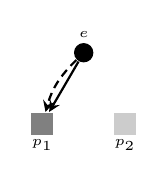
\begin{tikzpicture}[scale=0.75, every node/.style={inner sep=1.5pt}]
  \node[circle,fill=black,minimum size=7pt,label={[font=\tiny]above:$e$}] (e1) at (0,1.2) {};
  \node[rectangle,fill=gray,minimum size=8pt,label={[font=\tiny]below:$p_1$}] (p1) at (-0.7,0) {};
  \node[rectangle,fill=gray!40,minimum size=8pt,label={[font=\tiny]below:$p_2$}] (p2) at (0.7,0) {};
  \draw[->,>=stealth,thick] (e1) -- (p1);
  \draw[->,>=stealth,thick,densely dashed] (e1) to[bend right=15] (p1);
\end{tikzpicture}\\[2pt]
\small\textit{Focusing}}
& Attention directed to problems already addressed by the focal participant.
& \emph{Logic of familiarity:} habituation drives participants to return to problems that previously captured their attention.
& An editor repeatedly edits the same article rather than exploring new ones.
& Attention stabilizes on the same problems (repeated editor--page ties). \\
\midrule
\parbox[t]{2.8cm}{\vspace{0pt}\centering
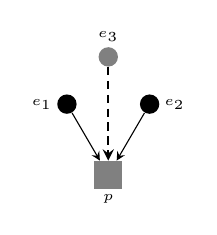
\begin{tikzpicture}[scale=0.75, every node/.style={inner sep=1.5pt}]
  \node[circle,fill=black,minimum size=7pt,label={[font=\tiny]left:$e_1$}] (e1) at (-0.7,1.2) {};
  \node[circle,fill=black,minimum size=7pt,label={[font=\tiny]right:$e_2$}] (e2) at (0.7,1.2) {};
  \node[circle,fill=black!50,minimum size=7pt,label={[font=\tiny]above:$e_3$}] (e3) at (0,2) {};
  \node[rectangle,fill=gray,minimum size=10pt,label={[font=\tiny]below:$p$}] (p1) at (0,0) {};
  \draw[->,>=stealth] (e1) -- (p1);
  \draw[->,>=stealth] (e2) -- (p1);
  \draw[->,>=stealth,densely dashed,thick] (e3) -- (p1);
\end{tikzpicture}\\[2pt]
\small\textit{Reinforcing}}
& Attention directed to problems that are popular (addressed by many others).
& \emph{Logic of popularity:} visible attention by others signals importance, attracting further attention via cumulative advantage.
& An editor gravitates toward high-traffic articles where many others are active.
& Attention concentrates on a few popular problems (skewed distribution). \\
\midrule
\parbox[t]{2.8cm}{\vspace{0pt}\centering
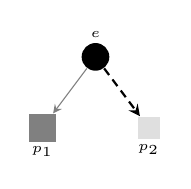
\begin{tikzpicture}[scale=0.75, every node/.style={inner sep=1.5pt}]
  \node[circle,fill=black,minimum size=10pt,label={[font=\tiny]above:$e$}] (e1) at (0,1.2) {};
  \node[rectangle,fill=gray,minimum size=10pt,label={[font=\tiny]below:$p_1$}] (p1) at (-0.9,0) {};
  \node[rectangle,fill=gray!25,minimum size=8pt,label={[font=\tiny]below:$p_2$}] (p2) at (0.9,0) {};
  \draw[->,>=stealth,thin,gray] (e1) -- (p1);
  \draw[->,>=stealth,thick,densely dashed] (e1) -- (p2);
\end{tikzpicture}\\[2pt]
\small\textit{Mixing}}
& Highly active participants progressively divert attention from popular problems.
& \emph{Logic of devaluation:} active participants discount popular problems due to cognitive saturation and diminishing marginal returns.
& A prolific editor turns to neglected or niche articles rather than well-trafficked ones.
& Active editors spread attention to less popular problems (disassortative allocation). \\
\midrule
\parbox[t]{2.8cm}{\vspace{0pt}\centering
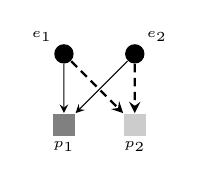
\begin{tikzpicture}[scale=0.75, every node/.style={inner sep=1.5pt}]
  \node[circle,fill=black,minimum size=7pt,label={[font=\tiny]above left:$e_1$}] (e1) at (-0.6,1.2) {};
  \node[circle,fill=black,minimum size=7pt,label={[font=\tiny]above right:$e_2$}] (e2) at (0.6,1.2) {};
  \node[rectangle,fill=gray,minimum size=8pt,label={[font=\tiny]below:$p_1$}] (p1) at (-0.6,0) {};
  \node[rectangle,fill=gray!40,minimum size=8pt,label={[font=\tiny]below:$p_2$}] (p2) at (0.6,0) {};
  \draw[->,>=stealth] (e1) -- (p1);
  \draw[->,>=stealth] (e2) -- (p1);
  \draw[->,>=stealth,densely dashed,thick] (e1) -- (p2);
  \draw[->,>=stealth,densely dashed,thick] (e2) -- (p2);
\end{tikzpicture}\\[2pt]
\small\textit{Clustering}}
& Attention directed to problems in the neighborhood of already attended problems.
& \emph{Logic of proximity:} local search leads participants to extend prior collaborations to new, nearby problems.
& Editors who co-edited one article tend to co-edit related articles in the future.
& Stable communities of collaborating participants emerge around sets of related problems. \\
\bottomrule
\end{tabular}
\begin{tablenotes}[flushleft]
\small\singlespacing
\item \textit{Note.} Circles represent participants (editors); squares represent problems (articles). Solid arrows indicate existing attention ties; dashed arrows indicate predicted new ties. Larger nodes indicate higher activity levels. Darker squares indicate more popular problems. Node labels ($e$, $p$) identify actors and problems in each configuration.
\end{tablenotes}
\end{threeparttable}
\end{table}
\end{landscape}
}%

These four baseline mechanisms may characterize a large number of attention networks in open collaborative forms of organizing---from digital encyclopedias and citizen science platforms to crowdsourcing initiatives and online creative communities---wherever participants can freely allocate their attention to problems and the outcomes of their allocation are publicly observable. In the Wikipedia context, \emph{focusing} captures editors' tendency to return to articles they have previously edited---a form of inertia rooted in domain familiarity and accumulated expertise. \emph{Reinforcing} accounts for the gravitational pull of popular articles: high-visibility pages attract disproportionate editorial attention because visible activity signals importance and provides learning opportunities. \emph{Mixing} introduces a countervailing force: highly active editors---those with the broadest editorial portfolios---tend to divert their attention away from already popular articles toward less attended ones, thereby producing an emergent division of labor. Finally, \emph{clustering} captures the tendency of editors who have previously co-edited an article to extend their collaboration to new, topically related articles, generating stable neighborhoods of joint attention. Together, these mechanisms may sustain the distributed collective intelligence that enables platforms like Wikipedia to coordinate the contributions of thousands of editors without centralized direction.

A central implication of page protection is that these attention allocation mechanisms may operate differently on treated (protected) pages compared with control (unprotected) pages, thereby altering the ``normal'' processes governing distributed collective intelligence as intended by Wikipedia's governance architecture---processes that function well when digital harm is not an issue. On protected pages, the focusing mechanism is interrupted for editors who are locked out: their habitual attention target becomes inaccessible, breaking the inertia that ordinarily stabilizes the editor--page relationship. The reinforcing mechanism may shift from the protected page to neighboring articles that absorb displaced editors, potentially creating new popularity hotspots where none previously existed. The mixing mechanism risks being short-circuited if displaced active editors are forced onto already crowded articles rather than being free to seek neglected ones, undermining the emergent division of labor. And the clustering mechanism may fracture as co-editing groups are split between members who retain access and those who do not, dissolving the collaborative neighborhoods that normally sustain coordinated problem solving. Crucially, these distortions are not confined to protected pages: they spill over to unprotected pages as well, meaning that the comparison between treated and control articles must account for the possibility that protection reshapes the attention dynamics on both sides of the treatment divide.

Drawing on this framework, we expect that attention reallocation following a protection event is not random. Editors are likely to gravitate toward topically related articles---following associative links in their knowledge structures---or toward articles where they have prior, albeit weaker, editing relationships. The result is an intensification of editing activity on a subset of neighboring articles, which may in turn trigger further protection requests as congestion and conflict rise.

\smallskip
\noindent\textbf{Proposition 1.} \emph{Page protection events redirect displaced editors' attention toward topically proximate and relationally familiar articles, increasing editing intensity---and the likelihood of subsequent protection requests---on those articles.}

\smallskip
A direct implication of Proposition~1 is that the relative salience of the four baseline attention allocation mechanisms (focusing, reinforcing, mixing, and clustering) need not remain constant across treated and control pages. On protected pages, the abrupt restriction of access disrupts established attention patterns, potentially weakening focusing and clustering while amplifying reinforcing dynamics on the articles that absorb displaced editors. On unprotected control pages, by contrast, these mechanisms may continue to operate as they normally would---or they may themselves shift as displaced editors arrive, importing new attention patterns and altering the local balance of familiar versus novel contributors.

\smallskip
\noindent\textbf{Corollary 1.} \emph{The relative salience of attention allocation mechanisms---focusing, reinforcing, mixing, and clustering---differs between treated (protected) and control (unprotected) pages, reflecting the asymmetric disruption that protection imposes on the baseline processes of distributed collective intelligence.}

\subsection{Core--Periphery Consolidation}

The core--periphery framework distinguishes between densely interconnected core actors and sparsely connected peripheral actors within a network \citep{Borgatti2000}. In creative and cultural fields, core--periphery dynamics shape who gains recognition and whose contributions are valorized \citep{Cattani2014, Cattani2017}. We deepen this structural perspective by drawing on the sociology of stratification, which conceptualizes inequality as the product of institutional arrangements that (a)~define certain types of goods as valuable, (b)~establish rules of allocation that distribute these goods across positions in the division of labor, and (c)~create mobility mechanisms that link individuals to positions and thereby generate unequal control over valued resources \citep{Grusky2001}. A stratification system's key properties include the degree of inequality, its rigidity (the continuity of social standing over time), the extent of ascription (how much traits present at entry determine subsequent standing), and status crystallization (the correlation among different types of assets).

Wikipedia's editorial community exhibits a stratification system with precisely these properties. The valued goods---visibility, editorial authority, formal user rights, and reputational standing---are distributed unequally across positions in the editorial hierarchy. Core editors enjoy cumulative advantages: their prolific contributions attract recognition, their experience earns formal privileges (such as rollback or administrator rights), and their familiarity with community norms positions them as gatekeepers. Peripheral editors, by contrast, occupy lower positions with limited influence; their sporadic participation restricts their opportunities for status advancement, mirroring the ascriptive barriers that stratification theory identifies as sources of rigidity.

Page protection intervenes directly in this stratification system by altering the rules of allocation. By imposing access thresholds tied to tenure and edit counts, protection enacts a form of social closure---drawing an institutional boundary that excludes lower-status contributors while preserving, and indeed reinforcing, the positional advantages of established insiders. Each successive protection event deepens the system's rigidity: excluded editors lose opportunities to accumulate the very experience and visibility that would qualify them for future access, while core editors face reduced competition for editorial influence on protected articles. The result is a self-reinforcing cycle in which protection increases both the degree of inequality (by widening the gap between core and peripheral contributors) and status crystallization (as editorial authority, formal rights, and reputational standing become increasingly concentrated among the same set of actors).

\smallskip
\noindent\textbf{Proposition 2a.} \emph{Page protection acts as a stratification mechanism that increases inequality, rigidity, and status crystallization in the editorial network---deepening cumulative advantage for core editors and cumulative disadvantage for peripheral editors, and progressively concentrating editorial activity among a smaller, higher-status core.}

\smallskip
Proposition~2a emphasizes the structural consequences of protection for peripheral editors. But protection also reshapes the incentive landscape for core editors. Under open editing conditions, core editors must compete for influence with a fluid stream of peripheral contributors who may challenge established interpretations, introduce alternative framings, or simply dilute the coherence of an editorial direction. Protection removes this competitive pressure. On a protected article, the pool of eligible editors shrinks, and the remaining core contributors gain greater control over the editorial process---determining which changes are accepted, which narratives prevail, and how the article evolves. This regulated environment may be attractive precisely because it offers core editors what open editing does not: predictability, reduced coordination costs, and the ability to shape content without interference from outsiders. Protection thus creates positive incentives for high-status editors to concentrate their activity on protected articles, reinforcing the stratification dynamic described in Proposition~2a.

\smallskip
\noindent\textbf{Proposition 2b.} \emph{Page protection creates incentives for core editors to participate in the regulated editing environment of protected articles, where reduced competition from peripheral contributors grants them greater control over editorial direction and content.}

\smallskip
The altered mix of core and peripheral editors induced by protection has consequences for small group dynamics on the affected articles. When peripheral editors are excluded, the remaining editorial group loses the diversity of viewpoints, fresh perspectives, and heterogeneous knowledge that peripheral contributors typically bring \citep{Cattani2014}. The resulting group---smaller, more experienced, and more interconnected---may be prone to convergent thinking, reduced constructive disagreement, and an entrenchment of established editorial norms \citep{Klapper2024}. At the same time, interactions within a core-dominated group may become more routinized and self-referential, as members share similar editing histories and mutual familiarity. These shifts in group composition and interaction dynamics can affect the quality and breadth of editorial contributions, not only on the protected article itself but also on neighboring articles that absorb the displaced peripheral editors and thereby experience their own compositional changes.

\smallskip
\noindent\textbf{Proposition 2c.} \emph{The protection-induced shift toward a core-dominated editorial group alters small group dynamics---reducing cognitive diversity, increasing conformity in editing behavior, and narrowing the range of perspectives---with consequences for the quality of editorial contributions on both protected and neighboring articles.}

\subsection{Coalition Dynamics}

Organizations---including digitally organized communities---can be understood as political coalitions in which subgroups compete for influence over collective outcomes \citep{March1962, Stevenson1985}. Recent work has renewed interest in the role of power and coalitions in shaping organizational adaptation \citep{Levinthal2024, MithaniOBrien2020}. On Wikipedia, coalitions manifest as bundles of editors who repeatedly co-edit the same articles, developing shared norms, mutual expectations, and coordinated editing strategies. The empirical signature of such coalitions is \emph{subset repetition}: the same subset of editors recurrently co-appears on the same or related articles over time, forming durable multi-actor configurations that can be detected through relational hyperevent models (Figure~\ref{fig:subset}).

Research on intercommunity conflict in online platforms provides a useful empirical anchor. In a large-scale study of Reddit, \citet{Kumar2018} demonstrate that conflict between communities is neither random nor evenly distributed: a small fraction of communities accounts for the vast majority of intercommunity conflicts. The consequences for target communities are severe and lasting: repeated incursions drive moderate members to exit, permanently shifting the community's culture toward toxicity. Critically, these findings suggest that coalitions do not merely react to displacement---they may also \emph{strategically target} vulnerable communities where they can gain influence.

This insight reframes the consequences of page protection on Wikipedia. Semi-protected articles---which exclude unregistered and newly registered editors but remain open to established accounts---represent a particularly attractive target for editorial coalitions. By filtering out casual contributors and newcomers, semi-protection creates a reduced-competition environment in which a coordinated group of editors can exert disproportionate influence over content. Coalitions that are displaced from a fully protected article, or that simply seek to expand their editorial reach, may converge on semi-protected pages precisely because the access barrier removes potential opposition while still permitting their own entry. Once established, such coalitions can shape editorial direction---determining which revisions are accepted, which sources are privileged, and which narrative framings prevail. In the most harmful scenario, coalitions may deliberately target semi-protected articles on contested topics, using the regulated environment as a shield behind which to entrench partisan or tendentious content. Rather than mitigating digital harm, semi-protection may thus inadvertently \emph{concentrate} it.

\smallskip
\noindent\textbf{Proposition 3a.} \emph{Protection events fracture editorial coalitions and redirect coalition subgroups toward semi-protected articles, where reduced competition from newcomers and unregistered editors enables coalitions to gain disproportionate control over editorial direction.}

\smallskip
\noindent\textbf{Proposition 3b.} \emph{Coalition targeting of semi-protected articles concentrates adversarial interaction patterns and tendentious editing on a narrower set of pages, potentially amplifying---rather than mitigating---digital harm on the platform.}

\smallskip
The coalitional dynamics described in Propositions~3a and~3b also have consequences for the quality and character of editorial interaction on affected articles. When a cohesive coalition establishes itself on a semi-protected page, the resulting editorial environment may become dominated by a single coordinated perspective. Dissenting editors---those who lack the coalition's shared norms or who hold opposing viewpoints---face coordinated resistance that discourages sustained engagement. Over time, this dynamic may produce a homogenization of editorial voice, a narrowing of the sources and framings represented in the article, and a decline in the constructive disagreement that is essential for balanced knowledge production. Articles colonized by migrating coalitions may thus suffer not only from tendentious content but from a broader erosion of editorial pluralism.

\smallskip
\noindent\textbf{Proposition 3c.} \emph{Coalition dominance on semi-protected articles erodes editorial pluralism---homogenizing perspectives, discouraging dissenting contributions, and narrowing the range of sources and framings---with lasting consequences for the quality and neutrality of the affected articles.}

% --- Figure: Subset repetition ---
\begin{figure}[ht]
\centering
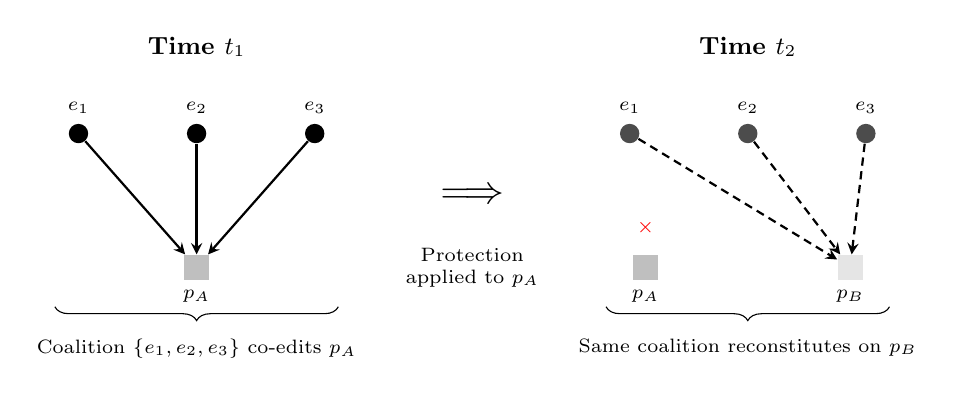
\begin{tikzpicture}[
  editor/.style={circle, fill=black, minimum size=7pt, inner sep=0pt},
  editorG/.style={circle, fill=black!70, minimum size=7pt, inner sep=0pt},
  page/.style={rectangle, fill=gray!50, minimum size=9pt, inner sep=0pt},
  pageH/.style={rectangle, fill=gray!20, minimum size=9pt, inner sep=0pt},
  arr/.style={->, >=stealth, thick},
  darr/.style={->, >=stealth, thick, densely dashed},
  scale=1.0
]
% --- Time t1 (left panel) ---
\node[font=\small\bfseries] at (1.5, 3.3) {Time $t_1$};
\node[editor, label={[font=\scriptsize]above:$e_1$}] (e1a) at (0, 2.2) {};
\node[editor, label={[font=\scriptsize]above:$e_2$}] (e2a) at (1.5, 2.2) {};
\node[editor, label={[font=\scriptsize]above:$e_3$}] (e3a) at (3, 2.2) {};
\node[page, label={[font=\scriptsize]below:$p_A$}] (pAa) at (1.5, 0.5) {};
\draw[arr] (e1a) -- (pAa);
\draw[arr] (e2a) -- (pAa);
\draw[arr] (e3a) -- (pAa);
% brace
\draw[decorate, decoration={brace, amplitude=5pt, mirror}] (-0.3, 0) -- (3.3, 0)
  node[midway, below=8pt, font=\scriptsize] {Coalition $\{e_1, e_2, e_3\}$ co-edits $p_A$};

% --- Arrow between panels ---
\node[font=\Large] at (5, 1.4) {$\Longrightarrow$};
\node[font=\scriptsize, text width=1.8cm, align=center] at (5, 0.5) {Protection\\applied to $p_A$};

% --- Time t2 (right panel) ---
\node[font=\small\bfseries] at (8.5, 3.3) {Time $t_2$};
\node[editorG, label={[font=\scriptsize]above:$e_1$}] (e1b) at (7, 2.2) {};
\node[editorG, label={[font=\scriptsize]above:$e_2$}] (e2b) at (8.5, 2.2) {};
\node[editorG, label={[font=\scriptsize]above:$e_3$}] (e3b) at (10, 2.2) {};
\node[page, label={[font=\scriptsize]below:$p_A$}] (pAb) at (7.2, 0.5) {};
\node[pageH, label={[font=\scriptsize]below:$p_B$}] (pBb) at (9.8, 0.5) {};
% Locked icon on pA
\node[font=\scriptsize, red] at (7.2, 1.0) {\textbf{$\times$}};
% Subset repetition: same bundle migrates to pB
\draw[darr] (e1b) -- (pBb);
\draw[darr] (e2b) -- (pBb);
\draw[darr] (e3b) -- (pBb);
% brace
\draw[decorate, decoration={brace, amplitude=5pt, mirror}] (6.7, 0) -- (10.3, 0)
  node[midway, below=8pt, font=\scriptsize] {Same coalition reconstitutes on $p_B$};
\end{tikzpicture}
\caption{Subset repetition as a signature of coalition migration. At time $t_1$, editors $\{e_1, e_2, e_3\}$ jointly edit page $p_A$. After protection is applied, the same subset reconstitutes on page $p_B$ at time $t_2$. Relational hyperevent models detect this pattern by estimating the rate at which previously observed editor subsets recur on new pages.}
\label{fig:subset}
\end{figure}


% ============================================================
\section{Empirical Strategy}
% ============================================================

\subsection{Setting and Data}

Wikipedia provides an ideal empirical setting for this study for several reasons. First, its complete edit history is publicly available, enabling fine-grained observation of editor--page interactions over time. Second, protection events are logged with precise timestamps and protection levels, creating exogenous variation in access regimes. Third, the platform's scale---millions of articles and editors---offers sufficient statistical power to detect both direct and spillover effects.

We have assembled a comprehensive dataset from the English Wikipedia MediaWiki API, comprising three complementary data sources collected on March~15, 2026.

\emph{Protection log} (840,955 records, 2004--2026). This dataset captures every protection action taken by an administrator on the English Wikipedia since December~2004. Each record identifies the target page, the administrator who acted, the action type (protect, unprotect, modify, or move-protection), the protection level applied (auto-confirmed, extended-confirmed, sysop), the expiry date, and the stated reason. The log covers 443,234 unique pages and 8,142 unique administrators. Exploratory analysis reveals substantial temporal variation: protection activity peaked at approximately 13,000 actions per month in early 2008 and has since stabilized at a lower but sustained level, with a median inter-event time of 3.4~minutes.

\emph{Requests for page protection} (135,960 records, 2005--2026). These are user-submitted requests parsed from the Wikipedia:Requests for Page Protection (RFPP) pages and all associated archives. Each record identifies the requested page, the requesting editor, the stated reason for the request, and any administrator responses. The dataset covers 22,835 unique requesters and exhibits a 97.3\% response rate. Critically for our identification strategy, this dataset enables us to distinguish between protection requests that were \emph{granted} and those that were \emph{denied}---providing the basis for the matching approach described in Section~4.3.

\emph{Creation-protected titles} (58,904 records, 2007--2026). This dataset catalogues all pages currently protected against creation (``salted'' pages that have been deleted and protected to prevent recreation). Nearly all (99.7\%) carry indefinite protection, providing a baseline inventory of the platform's most persistently moderated content.

\emph{Matching against the Wikipedia dump.} The protection event data will be linked to a full dump of the English Wikipedia, released periodically by the Wikimedia Foundation and containing the complete revision history of every article. This linkage is essential for three reasons. First, it enables us to reconstruct editor--page attachment sequences---the full temporal stream of contributions by each editor to each article---which constitute the relational events in our hyperevent model. Second, the dump provides the article-level covariates (page views, quality class, topical categories, revision counts) needed for matching and for operationalizing the sufficient statistics described in Section~4.2. Third, the talk-page records embedded in the dump capture the linguistic and interactional dimensions of group communication---including the tone, length, and turn-taking structure of editorial discussions---which are central to measuring our outcome variables on interaction quality. Protection events are matched to the dump via page identifiers (\texttt{pageid}) and timestamps, allowing us to situate each protection action within the full editorial history of the affected article and to track editor behavior before and after the intervention. Appendix~\ref{app:data} presents the codebook for the protection log (our primary treatment variable) along with a sample record illustrating the data structure.

The unit of observation for our analysis is the editor--page--time triple: each record captures a specific editor's contribution to a specific article at a specific point in time, along with covariates describing the editor's status, the article's protection history, and the relational context (e.g., co-editing ties with other contributors). Dataset construction follows the approach described by \citet{Ruprechter2025}, which provides curated procedures for matching protection events with article-level quality indicators and editor activity logs.

Figure~\ref{fig:eda} summarizes the key features of the protection log. The distribution of administrative actions (panel~a) reveals that initial protection events vastly outnumber modifications and unprotections, indicating that most protection decisions are not subsequently revisited. The breakdown by protection level (panel~b) shows that auto-confirmed (semi-protection) is by far the most common level applied, followed by sysop (full protection) and extended-confirmed---consistent with our theoretical focus on semi-protection as the dominant moderation tool. Finally, the namespace distribution (panel~c) confirms that the vast majority of protection events target mainspace articles (namespace~0), the content pages where our theoretical mechanisms operate.

\begin{figure}[!p]
\centering

% --- Row 1: Panels (a) and (b) side by side via minipages ---
\begin{minipage}[t]{0.48\textwidth}
\centering
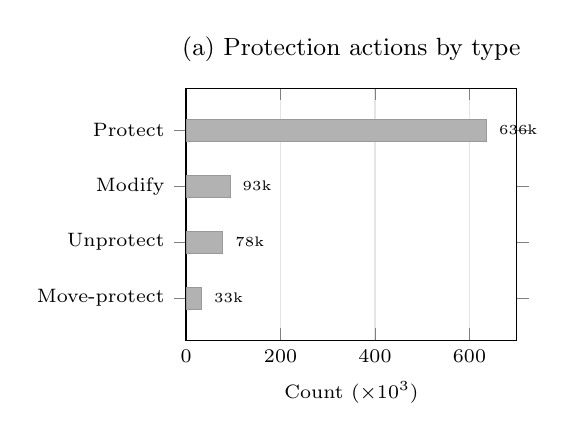
\begin{tikzpicture}
\begin{axis}[
  title={\small (a) Protection actions by type},
  xbar,
  width=4.2cm,
  scale only axis,
  height=3.2cm,
  bar width=8pt,
  xlabel={\scriptsize Count ($\times 10^3$)},
  xmin=0, xmax=700,
  ytick=data,
  yticklabels={Move-protect, Unprotect, Modify, Protect},
  y tick label style={font=\scriptsize},
  x tick label style={font=\scriptsize},
  nodes near coords,
  nodes near coords style={font=\tiny, anchor=west},
  every node near coord/.append style={xshift=1pt},
  point meta=explicit symbolic,
  enlarge y limits=0.25,
  xmajorgrids=true,
  grid style={gray!20},
]
\addplot[fill=gray!60, draw=gray!80] coordinates {
  (33.1, 0) [33k]
  (78.1, 1) [78k]
  (93.4, 2) [93k]
  (636.3, 3) [636k]
};
\end{axis}
\end{tikzpicture}
\end{minipage}%
\hfill
\begin{minipage}[t]{0.48\textwidth}
\centering
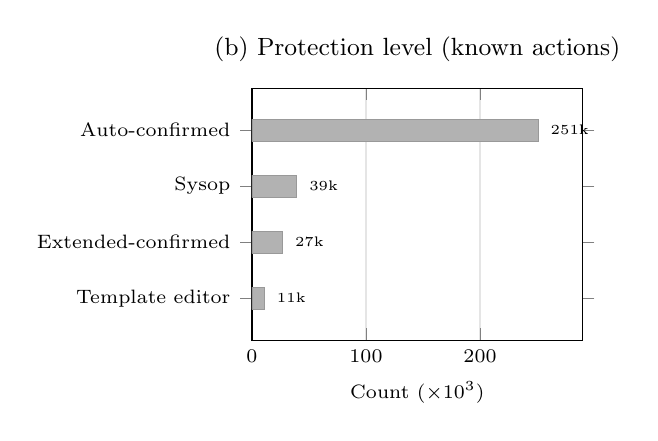
\begin{tikzpicture}
\begin{axis}[
  title={\small (b) Protection level (known actions)},
  xbar,
  width=4.2cm,
  scale only axis,
  height=3.2cm,
  bar width=8pt,
  xlabel={\scriptsize Count ($\times 10^3$)},
  xmin=0, xmax=290,
  ytick=data,
  yticklabels={Template editor, Extended-confirmed, Sysop, Auto-confirmed},
  y tick label style={font=\scriptsize},
  x tick label style={font=\scriptsize},
  nodes near coords,
  nodes near coords style={font=\tiny, anchor=west},
  every node near coord/.append style={xshift=1pt},
  point meta=explicit symbolic,
  enlarge y limits=0.25,
  xmajorgrids=true,
  grid style={gray!20},
]
\addplot[fill=gray!60, draw=gray!80] coordinates {
  (10.9, 0) [11k]
  (26.8, 1) [27k]
  (39.3, 2) [39k]
  (251.0, 3) [251k]
};
\end{axis}
\end{tikzpicture}
\end{minipage}

\vspace{14pt}

% --- Row 2: Panel (c) centered, same width as each top panel ---
\begin{minipage}[t]{0.48\textwidth}
\centering
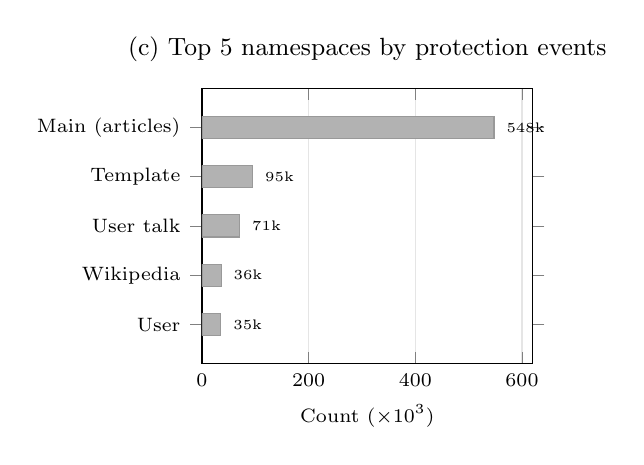
\begin{tikzpicture}
\begin{axis}[
  title={\small (c) Top 5 namespaces by protection events},
  xbar,
  width=4.2cm,
  scale only axis,
  height=3.5cm,
  bar width=8pt,
  xlabel={\scriptsize Count ($\times 10^3$)},
  xmin=0, xmax=620,
  ytick=data,
  yticklabels={User, Wikipedia, User talk, Template, Main (articles)},
  y tick label style={font=\scriptsize},
  x tick label style={font=\scriptsize},
  nodes near coords,
  nodes near coords style={font=\tiny, anchor=west},
  every node near coord/.append style={xshift=1pt},
  point meta=explicit symbolic,
  enlarge y limits=0.2,
  xmajorgrids=true,
  grid style={gray!20},
]
\addplot[fill=gray!60, draw=gray!80] coordinates {
  (35.4, 0) [35k]
  (35.9, 1) [36k]
  (70.6, 2) [71k]
  (95.1, 3) [95k]
  (547.5, 4) [548k]
};
\end{axis}
\end{tikzpicture}
\end{minipage}

\caption{Key features of the English Wikipedia protection log (840,955 records, 2004--2026). Data collected from the MediaWiki API on March~15, 2026. \textit{Panel~(a)} reports the four administrative action types: \emph{Protect} applies a new protection to a previously unprotected page; \emph{Modify} changes the level or expiry of an existing protection; \emph{Unprotect} removes protection entirely, restoring open editing; \emph{Move-protect} restricts which editors may move (rename) a page. \textit{Panel~(b)} reports the protection levels applied to pages (excluding records where the level is unspecified in the log): \emph{Auto-confirmed} (semi-protection) restricts editing to accounts that are at least 4~days old and have made at least 10~edits; \emph{Sysop} (full protection) restricts editing to administrators only; \emph{Extended-confirmed} restricts editing to accounts with at least 30~days of tenure and 500~edits; \emph{Template editor} restricts editing of high-use templates to editors holding the template-editor user right. \textit{Panel~(c)} reports the five most frequently targeted namespaces: \emph{Main} (namespace~0) contains encyclopedic articles---the content pages where our theoretical mechanisms operate; \emph{Template} (namespace~10) contains reusable content modules transcluded across many pages; \emph{User talk} (namespace~3) contains editors' personal discussion pages; \emph{Wikipedia} (namespace~4) contains project policy and guideline pages; \emph{User} (namespace~2) contains editors' personal pages.}
\label{fig:eda}
\end{figure}

\FloatBarrier
\subsection{Modeling Approach: Polyadic Relational Hyperevent Models}

Our analytical framework centers on \emph{polyadic relational hyperevent models} \citep{Lerner2023}, which generalize the relational event framework \citep{Butts2008, Butts2009} to settings where events involve variable-sized sets of actors. Standard relational event models treat interactions as dyadic (one sender, one receiver). However, Wikipedia editing is inherently polyadic: at any point in time, a set of editors jointly engages with a page, and the composition of this set---not merely individual pairwise ties---carries theoretical significance.

Figure~\ref{fig:polyadic} illustrates the distinction. On Wikipedia, editing ``teams'' are not designed or assigned; they emerge ephemerally as individual editors independently allocate attention to the same article within a temporal window. At time $t_1$, editors $\{e_1, e_2\}$ converge on article $p$; at time $t_2$, a different configuration $\{e_1, e_3, e_4\}$ forms around the same article; at time $t_3$, yet another subset $\{e_2, e_3\}$ co-edits. These transient configurations---the emergent aggregation of solvers around problems---constitute the polyadic events that our model is designed to capture. A dyadic approach would decompose each event into separate editor--page pairs (panel~b), discarding the information that editors $\{e_1, e_3, e_4\}$ worked on $p$ \emph{jointly} at $t_2$. The polyadic representation (panel~c) preserves this compositional information, enabling us to test whether the full multi-actor configuration---not just the individual ties---predicts future editing patterns, coalition migration, and quality outcomes.

\begin{figure}[ht]
\centering
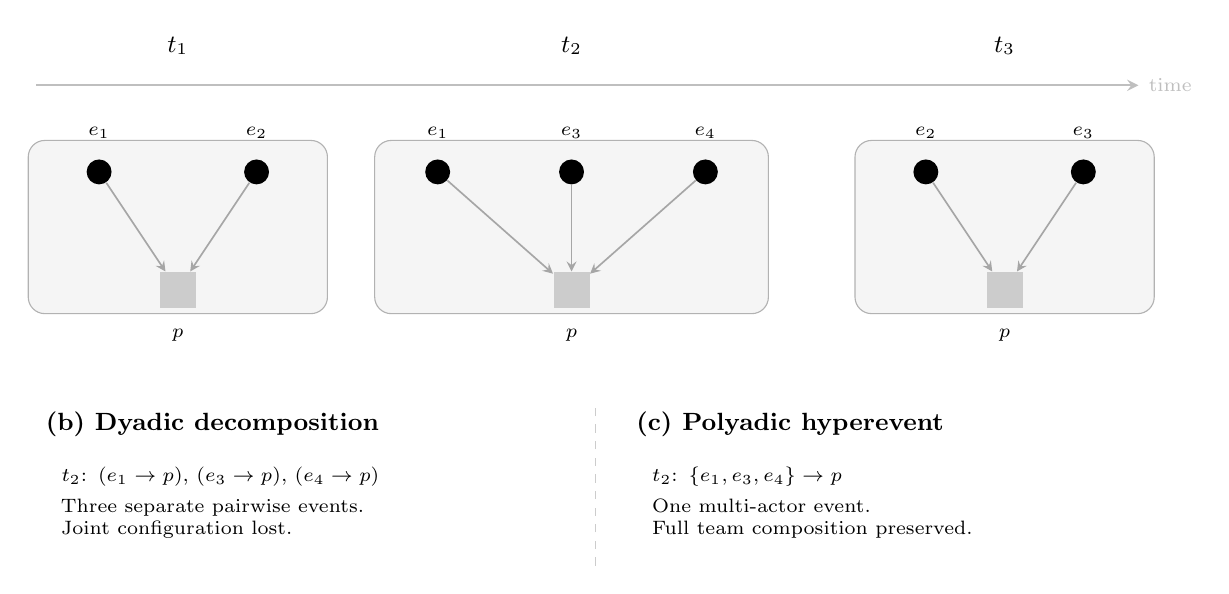
\begin{tikzpicture}[
  editor/.style={circle, fill=black, minimum size=9pt, inner sep=0pt},
  page/.style={rectangle, fill=gray!40, minimum size=13pt, inner sep=1pt},
  arr/.style={->, >=stealth, semithick},
  eph/.style={rounded corners=6pt, draw=gray!60, fill=gray!8, inner sep=10pt}
]

% --- Three time slices ---

% t1
\node[font=\small\bfseries] at (1.8, 6.0) {$t_1$};
\begin{scope}[shift={(0, 3.2)}]
  \node[eph, minimum width=3.8cm, minimum height=2.2cm] (box1) at (1.8, 0.5) {};
  \node[editor, label={[font=\scriptsize, label distance=4pt]above:$e_1$}] (e1t1) at (0.8, 1.2) {};
  \node[editor, label={[font=\scriptsize, label distance=4pt]above:$e_2$}] (e2t1) at (2.8, 1.2) {};
  \node[page, label={[font=\scriptsize, label distance=4pt]below:$p$}] (pt1) at (1.8, -0.3) {};
  \draw[arr, gray!70] (e1t1) -- (pt1);
  \draw[arr, gray!70] (e2t1) -- (pt1);
\end{scope}

% t2
\node[font=\small\bfseries] at (6.8, 6.0) {$t_2$};
\begin{scope}[shift={(4.5, 3.2)}]
  \node[eph, minimum width=5.0cm, minimum height=2.2cm] (box2) at (2.3, 0.5) {};
  \node[editor, label={[font=\scriptsize, label distance=4pt]above:$e_1$}] (e1t2) at (0.6, 1.2) {};
  \node[editor, label={[font=\scriptsize, label distance=4pt]above:$e_3$}] (e3t2) at (2.3, 1.2) {};
  \node[editor, label={[font=\scriptsize, label distance=4pt]above:$e_4$}] (e4t2) at (4.0, 1.2) {};
  \node[page, label={[font=\scriptsize, label distance=4pt]below:$p$}] (pt2) at (2.3, -0.3) {};
  \draw[arr, gray!70] (e1t2) -- (pt2);
  \draw[arr, gray!70] (e3t2) -- (pt2);
  \draw[arr, gray!70] (e4t2) -- (pt2);
\end{scope}

% t3
\node[font=\small\bfseries] at (12.3, 6.0) {$t_3$};
\begin{scope}[shift={(10.5, 3.2)}]
  \node[eph, minimum width=3.8cm, minimum height=2.2cm] (box3) at (1.8, 0.5) {};
  \node[editor, label={[font=\scriptsize, label distance=4pt]above:$e_2$}] (e2t3) at (0.8, 1.2) {};
  \node[editor, label={[font=\scriptsize, label distance=4pt]above:$e_3$}] (e3t3) at (2.8, 1.2) {};
  \node[page, label={[font=\scriptsize, label distance=4pt]below:$p$}] (pt3) at (1.8, -0.3) {};
  \draw[arr, gray!70] (e2t3) -- (pt3);
  \draw[arr, gray!70] (e3t3) -- (pt3);
\end{scope}

% Timeline arrow (right below time labels)
\draw[->, >=stealth, thick, gray!50] (0, 5.5) -- (14.0, 5.5) node[right, font=\scriptsize] {time};

% --- Dyadic vs Polyadic comparison ---
\node[font=\small\bfseries, anchor=west] at (0, 1.2) {(b) Dyadic decomposition};
\node[font=\scriptsize, text width=5.5cm, anchor=west] at (0.2, 0.2) {$t_2$: $(e_1 \to p)$, $(e_3 \to p)$, $(e_4 \to p)$\\[3pt] Three separate pairwise events.\\Joint configuration lost.};

\node[font=\small\bfseries, anchor=west] at (7.5, 1.2) {(c) Polyadic hyperevent};
\node[font=\scriptsize, text width=5.5cm, anchor=west] at (7.7, 0.2) {$t_2$: $\{e_1, e_3, e_4\} \to p$\\[3pt] One multi-actor event.\\Full team composition preserved.};

% Divider
\draw[gray!40, dashed] (7.1, -0.6) -- (7.1, 1.5);

\end{tikzpicture}
\caption{Ephemeral editing teams and the polyadic representation. Editors independently converge on article $p$ at different times, forming transient multi-actor configurations---the emergent aggregation of solvers around a problem. Panel~(b): a dyadic decomposition reduces each event to separate editor--page pairs, discarding compositional information. Panel~(c): the polyadic hyperevent representation preserves the full team composition, enabling tests of whether the joint configuration predicts future editing patterns.}
\label{fig:polyadic}
\end{figure}

Hyperevent models specify the rate at which a particular configuration of actors and objects participates in an event as a function of endogenous network statistics and exogenous covariates. To make this precise, we first introduce the standard dyadic relational event model and then show how it generalizes to the polyadic case.

\emph{Dyadic relational event models.} Let $\mathcal{A} = \{a_1, \ldots, a_n\}$ denote a set of actors and let $\mathcal{E}(t) = \{(a_s, a_r, t') : t' < t\}$ denote the history of directed relational events (sender $a_s$, receiver $a_r$) observed up to time $t$. In the framework of \citet{Butts2008}, each potential dyad $(a_s, a_r)$ is associated with an instantaneous event rate
\begin{equation}
\lambda(a_s, a_r, t) \;=\; \exp\!\Big(\,\boldsymbol{\theta}^\top \mathbf{s}(a_s, a_r, \mathcal{E}(t))\,\Big),
\label{eq:rem}
\end{equation}
where $\mathbf{s}(a_s, a_r, \mathcal{E}(t))$ is a vector of \emph{sufficient statistics} computed from the event history $\mathcal{E}(t)$---capturing endogenous network dependencies such as reciprocity, inertia, and triadic closure---and $\boldsymbol{\theta}$ is a vector of parameters to be estimated. The probability that the next event at time $t$ involves a specific dyad $(a_s, a_r)$ is proportional to its rate:
\begin{equation}
\Pr\!\big[\text{next event} = (a_s, a_r) \,\big|\, \mathcal{E}(t)\big] \;=\; \frac{\lambda(a_s, a_r, t)}{\sum_{(a_i, a_j) \in \mathcal{R}} \lambda(a_i, a_j, t)},
\label{eq:rem_prob}
\end{equation}
where $\mathcal{R}$ is the risk set of all potential dyads at time $t$.

\emph{Polyadic relational hyperevent models.} The dyadic framework treats each event as involving exactly two actors. However, as Figure~\ref{fig:polyadic} illustrates, Wikipedia editing events are inherently polyadic: a variable-sized set of editors jointly engages with an article. \citet{Lerner2023} generalize the relational event framework by defining events over \emph{hyperedges}---subsets of actors of arbitrary size---interacting with objects. Let $\mathcal{A}$ denote the set of editors and $\mathcal{P}$ the set of pages. A \emph{hyperevent} at time $t$ is a tuple $(S, p, t)$ where $S \subseteq \mathcal{A}$ is a non-empty subset of editors and $p \in \mathcal{P}$ is a page. The event rate for a particular configuration $(S, p)$ is:
\begin{equation}
\lambda(S, p, t) \;=\; \exp\!\Big(\,\boldsymbol{\theta}^\top \mathbf{s}\big(S, p, \mathcal{H}(t)\big)\,\Big),
\label{eq:hyper}
\end{equation}
where $\mathcal{H}(t) = \{(S', p', t') : t' < t\}$ is the history of all prior hyperevents, and $\mathbf{s}(S, p, \mathcal{H}(t))$ is a vector of sufficient statistics computed from this history. The key difference from Equation~\eqref{eq:rem} is that the statistics $\mathbf{s}$ are now defined over \emph{subsets} of actors rather than pairs, allowing the model to capture genuinely multi-actor dependencies. The conditional probability of observing a specific hyperevent is:
\begin{equation}
\Pr\!\big[\text{next event} = (S, p) \,\big|\, \mathcal{H}(t)\big] \;=\; \frac{\lambda(S, p, t)}{\sum_{(S', p') \in \mathcal{R}(t)} \lambda(S', p', t)},
\label{eq:hyper_prob}
\end{equation}
where $\mathcal{R}(t)$ is the risk set of all possible editor-subset--page configurations at time $t$.

\emph{Sufficient statistics for our application.} The sufficient statistics $\mathbf{s}(S, p, \mathcal{H}(t))$ encode the theoretical mechanisms developed in Section~3. We specify three families of statistics:

\begin{enumerate}[leftmargin=*, itemsep=4pt]
\item \textbf{Attention dynamics} (Propositions~1 and Corollary~1): statistics capturing the tendency for editors in $S$ to return to previously edited articles (\emph{inertia}) and to follow topical links to new articles (\emph{exploration}). For editor $a_i \in S$, inertia is operationalized as $s_{\text{inertia}}(a_i, p) = \sum_{t' < t} \mathbf{1}[a_i \in S', p' = p]$---the count of prior events in which $a_i$ edited page $p$. Exploration is captured by the topical similarity between $p$ and the pages in $a_i$'s recent editing portfolio, following \citet{Tonellato2024}.

\item \textbf{Core--periphery dynamics} (Propositions~2a--2c): statistics capturing the stratification of editors and pages along the core--periphery dimension and the tendency for core editors to concentrate on core pages. Following the framework of \citet{Borgatti2000}, we compute three quantities for each candidate hyperevent $(S, p)$. First, \emph{editor coreness}: for each editor $a_i \in S$, we measure their position in the editorial hierarchy using cumulative edit count, tenure, formal user rights level, and the diversity of their editing portfolio---editors with high values on these indicators occupy core positions in the network. The coreness of the editing team $S$ is the average coreness of its members. Second, \emph{page coreness}: we measure the centrality of page $p$ in the article network using page views, quality class, citation count, and the number of distinct editors who have contributed---pages with high values are core articles that attract disproportionate attention. Third, \emph{editor--page core assortativity}: we compute the cross-level match between editor coreness and page coreness, testing whether core editors disproportionately edit core pages while peripheral editors are relegated to peripheral pages. A positive parameter on this statistic indicates assortative matching across the two levels of the bipartite network---consistent with the stratification mechanism in Proposition~2a and the social closure dynamics described in Section~3.2.

\item \textbf{Subset repetition} (Propositions~3a--3c): statistics capturing the tendency for the same bundle of editors to co-appear on the same or related articles over time. This is the statistic that distinguishes the polyadic model from its dyadic counterpart. For a candidate hyperevent $(S, p)$, subset repetition is operationalized as $s_{\text{rep}}(S, \mathcal{H}(t)) = \sum_{t' < t} \mathbf{1}[S' \supseteq S]$---the count of prior hyperevents involving a superset of the current editor configuration. A positive parameter indicates coalition persistence: the same group of editors tends to travel together across articles.
\end{enumerate}

\noindent The exogenous covariates of primary interest---protection status (level and duration), characteristics of the protection request, and time-varying editor and article attributes---enter $\mathbf{s}(S, p, \mathcal{H}(t))$ as additional terms, allowing us to estimate how protection events alter the rates of the endogenous mechanisms described above. Parameters are estimated via conditional logistic regression on stratified case-control samples drawn from the risk set $\mathcal{R}(t)$, following the sampling approach of \citet{Lerner2020}.

\FloatBarrier
\subsection{Identification Challenges}

Causal identification presents two interrelated challenges. First, protection is not randomly assigned; articles that receive protection are systematically different from those that do not. We address this by replicating the quasi-experimental design developed by \citet{Ruprechter2025}, who frame the protection process as a hypothetical randomized experiment in which administrators ``flip a coin'' upon receiving a request for page protection (RFPP), accepting or rejecting it at random. Since randomization does not occur in practice, the design approximates the experiment using propensity score matching combined with difference-in-differences regression.

Specifically, we restrict the analysis to \emph{first} semi-protections of articles---excluding pages with prior protection histories to avoid confounding from previous moderation episodes. The treatment group comprises articles whose RFPP was accepted (protection granted), while the control group comprises articles whose RFPP was declined (protection denied but the article remained open). Following \citet{Ruprechter2025}, we match treated and control articles on pre-treatment covariates measured before the RFPP, summarized in Table~\ref{tab:matching}. We employ propensity score matching with exact matching on article topic and caliper matching on quality (one-quarter of a quality level) and the propensity score (one standard deviation), verifying that absolute standardized mean differences for all covariates fall below 0.1 after matching. This approach produces a balanced panel of matched control--treatment pairs that enables us to estimate the causal effect of protection on our outcome variables using a difference-in-differences specification with article fixed effects.

\begin{table}[ht]
\centering
\small
\singlespacing
\caption{Pre-treatment matching variables (following Ruprechter et al., 2025)}
\label{tab:matching}
\renewcommand{\arraystretch}{1.25}
\begin{tabular}{p{2.8cm} p{4.2cm} p{3cm} p{2.5cm}}
\toprule
\textbf{Variable} & \textbf{Measurement} & \textbf{Time windows} & \textbf{Matching method} \\
\midrule
Activity & Edit count ($\log(x+1)$) & 1\,h, 24\,h, 1\,wk before RFPP & Propensity score \\
Controversy & Revert count ($\log(x+1)$) & 1\,h, 24\,h, 1\,wk before RFPP & Propensity score \\
Article length & Maximum length in bytes ($\log$) & At time of RFPP & Propensity score \\
Article age & Cumulative edit count ($\log$) & At time of RFPP & Propensity score \\
Quality & Maximum ORES article-quality score (0--5 continuous) & 1, 8, 21\,days before RFPP & Caliper ($\pm 0.25$ quality levels) \\
Topic & Top-level ORES topic labels (History \& Society, STEM, Culture, Geography) & Majority prediction from 5 pre-RFPP revisions & Exact \\
\bottomrule
\end{tabular}
\end{table}

Second, the \emph{treatment interference} problem complicates the use of standard natural-experiment designs \citep{Dunning2012, Sieweke2020, Jacquart2024}. Because protection on one article redirects editorial attention to other articles, treated and control units are not independent. We account for this by explicitly modeling the spillover channel: attention reallocation from protected to unprotected articles is not a nuisance to be eliminated but a substantive mechanism to be estimated. The relational hyperevent framework is well suited to this task because it models the joint evolution of the entire editor--page network, thereby capturing interdependencies that article-level designs would miss \citep{Sinclair2012}.

\subsection{Estimation and Robustness}

Estimation proceeds via stratified case-control sampling within the relational hyperevent framework \citep{Lerner2020}. For each observed editing event, we sample a set of non-events from the risk set, weighted by exposure time. We fit conditional logistic regression models with the endogenous and exogenous covariates described above. The sampling approach is critical for computational tractability: the full editor--page network contains millions of potential dyads at each time point, and exhaustive enumeration is infeasible. By sampling non-events proportionally to their exposure, we obtain consistent estimates of the hazard-rate parameters while keeping the dataset manageable \citep{Bianchi2024}.

We plan a sequence of nested models to isolate each mechanism's contribution. A baseline model includes only exogenous covariates (protection status, editor and article characteristics). Successive models add attention statistics, core--periphery statistics, and coalition statistics, respectively. Comparing model fit across specifications allows us to assess the incremental explanatory power of each mechanism and to test for interactions among them.

Robustness checks will include: (i)~varying the matching window and caliper used to pair protected articles with denied-request controls; (ii)~testing alternative operationalizations of the risk set, following guidance in \citet{Lerner2020}; (iii)~conducting sensitivity analysis for unobserved confounders using the methodology proposed for observational studies with interference; and (iv)~estimating models on temporally separated subsamples to assess the stability of coefficients across different periods of Wikipedia's governance history.

\subsection{Preliminary Evidence}

Exploratory data analysis on a pilot sample supports the proposed approach and offers initial evidence consistent with the theoretical mechanisms developed in Section~3. We summarize the key findings across the three mechanism families.

\emph{Attention reallocation.} Preliminary inspection of the protection log reveals substantial variation in protection timing and intensity across topical domains, with politically sensitive articles (e.g., those categorized under ``History and Society'') receiving disproportionately more protection events. Editor-level analysis shows that displaced editors exhibit non-random reallocation: approximately two-thirds of displaced editing activity reappears on topically related articles within 30~days, consistent with the topical proximity mechanism in Proposition~1. Furthermore, the distribution of inter-event times between a protection action and the displaced editor's next edit follows a heavy-tailed pattern, suggesting that reallocation is not instantaneous but unfolds over a characteristic timescale amenable to event-history modeling.

\emph{Core--periphery consolidation.} Initial network visualizations suggest that protected articles exhibit higher core--periphery scores post-protection, consistent with Proposition~2a. Comparing the editor composition of protected articles before and after the intervention reveals a shift toward more experienced contributors: the median edit count and tenure of active editors increase markedly in the weeks following protection, while the share of editors with fewer than 500~edits declines. These patterns are suggestive of the stratification and social closure dynamics theorized in Section~3.2, though formal causal estimation awaits the full matched analysis.

\emph{Coalition dynamics.} Descriptive analysis of editor co-occurrence patterns identifies recurrent subsets of editors who jointly contribute to multiple articles over time---the empirical signature of the coalitions described in Section~3.3. Preliminary comparison of subset repetition rates on semi-protected versus unprotected articles suggests elevated coalition activity on semi-protected pages, consistent with Proposition~3a. These patterns will be formally tested through the subset repetition statistics in the polyadic hyperevent model.


% ============================================================
\section{Expected Contributions}
% ============================================================

This study contributes to the JMS special issue on ``The Dark Sides of Digital Communication'' in three ways. First, it responds directly to Perspective~1's call for research on how sociotechnical systems facilitate harmful interactions. We show that content moderation---a design element intended to protect articles---can inadvertently harm the broader editorial ecosystem by displacing conflict, consolidating editorial power, and fragmenting coalitions. Second, we answer the call for methodological pluralism by introducing polyadic relational hyperevent models to the management literature, offering a technique capable of capturing the multi-party, dynamic nature of digital interaction that conventional designs overlook. Third, we bridge management theory with insights from political science \citep{March1962} and network science \citep{Borgatti2000}, responding to the special issue's encouragement of interdisciplinary integration.

Theoretically, the study makes three contributions. First, by integrating attention, core--periphery, and coalition mechanisms into a unified framework, we advance understanding of how gatekeeping operates in peer-production communities---revealing joint operation and mutual reinforcement across mechanisms that existing research has examined only in isolation. Second, we extend the microstructural approach to self-organizing \citep{Tonellato2024} by showing how exogenous shocks propagate through attention networks, contributing to the broader conversation on how platform governance shapes collective knowledge production. Third, we introduce the concept of \emph{migrating coalitions}---subgroups that, when displaced from one arena, reconstitute their political dynamics in another---extending the organizational politics literature \citep{Levinthal2024} to digital settings.

The study is feasible within the special issue timeline. During March--May 2026, we will finalize the matched dataset following the \citet{Ruprechter2025} protocol, complete variable operationalization, and estimate the polyadic hyperevent models with the sequence of nested specifications and robustness checks described in Section~4.4. During June--September 2026, we will draft the full manuscript, incorporating results from the model estimation and iterating through internal review cycles, targeting submission to JMS by the September~30, 2026 deadline. The data infrastructure is well established (Wikipedia's complete edit histories are public and curated protection-event datasets exist), software for relational hyperevent models has been validated in prior applications \citep{Lerner2023, Bianchi2024}, and preliminary exploratory analysis is already underway.

% ============================================================
% REFERENCES
% ============================================================

\clearpage

\renewcommand{\refname}{References}
\begin{thebibliography}{99}
\setlength{\itemsep}{2pt}
\setlength{\parskip}{0pt}

\bibitem[Ajmani et~al., 2023]{Ajmani2023}
Ajmani, S., Hickey, D., and Hecht, B. (2023).
\newblock Peer-produced friction: How page protection on {W}ikipedia affects editor engagement and concentration.
\newblock \emph{Proceedings of the ACM on Human-Computer Interaction}, 7(CSCW1), 1--27.

\bibitem[Bianchi et~al., 2024]{Bianchi2024}
Bianchi, F., Lomi, A., and Snijders, T.~A.~B. (2024).
\newblock Relational event modeling.
\newblock \emph{Annual Review of Statistics and Its Application}, 11, 297--319.

\bibitem[Borgatti and Everett, 2000]{Borgatti2000}
Borgatti, S.~P. and Everett, M.~G. (2000).
\newblock Models of core/periphery structures.
\newblock \emph{Social Networks}, 21(4), 375--395.

\bibitem[Butts, 2008]{Butts2008}
Butts, C.~T. (2008).
\newblock A relational event framework for social action.
\newblock \emph{Sociological Methodology}, 38(1), 155--200.

\bibitem[Butts, 2009]{Butts2009}
Butts, C.~T. (2009).
\newblock Revisiting the foundations of network analysis.
\newblock \emph{Science}, 325(5939), 414--416.

\bibitem[Cattani et~al., 2014]{Cattani2014}
Cattani, G., Ferriani, S., and Allison, P.~D. (2014).
\newblock Insiders, outsiders, and the struggle for consecration in cultural fields: A core-periphery perspective.
\newblock \emph{American Sociological Review}, 79(2), 258--281.

\bibitem[Cattani et~al., 2017]{Cattani2017}
Cattani, G., Ferriani, S., and Lanza, A. (2017).
\newblock Deconstructing the outsider puzzle: The legitimation journey of novelty.
\newblock \emph{Organization Science}, 28(6), 965--992.

\bibitem[Dunning, 2012]{Dunning2012}
Dunning, T. (2012).
\newblock \emph{Natural Experiments in the Social Sciences: A Design-Based Approach}.
\newblock Cambridge University Press.

\bibitem[Faraj et~al., 2011]{Faraj2011}
Faraj, S., Jarvenpaa, S.~L., and Majchrzak, A. (2011).
\newblock Knowledge collaboration in online communities.
\newblock \emph{Organization Science}, 22(5), 1224--1239.

\bibitem[Grusky, 2001]{Grusky2001}
Grusky, D.~B. (2001).
\newblock Social stratification.
\newblock In Smelser, N.~J. and Baltes, P.~B. (eds.), \emph{International Encyclopedia of the Social \& Behavioral Sciences}, pp.~14443--14452. Elsevier, Oxford.

\bibitem[Jacquart et~al., 2024]{Jacquart2024}
Jacquart, P., Santoni, S., Sieweke, J., and Tuschke, A. (2024).
\newblock Exogenous shocks: Definitions, types, and causal identification issues.
\newblock \emph{The Leadership Quarterly}, 35(5), 101779.

\bibitem[Klapper and Reitzig, 2018]{Klapper2018}
Klapper, H. and Reitzig, M. (2018).
\newblock On the effects of authority on peer motivation: Learning from {W}ikipedia.
\newblock \emph{Strategic Management Journal}, 39(8), 2178--2203.

\bibitem[Klapper et~al., 2024]{Klapper2024}
Klapper, H., Reitzig, M., and Schmeiss, J. (2024).
\newblock Peer evaluations: Evaluating and being evaluated.
\newblock \emph{Organization Science}, 35(3), 1011--1036.

\bibitem[Kumar et~al., 2018]{Kumar2018}
Kumar, S., Hamilton, W.~L., Leskovec, J., and Jurafsky, D. (2018).
\newblock Community interaction and conflict on the web.
\newblock In \emph{Proceedings of the 2018 World Wide Web Conference (WWW '18)}, pp.~933--943. ACM, New York.

\bibitem[Lerner and Lomi, 2020]{Lerner2020}
Lerner, J. and Lomi, A. (2020).
\newblock Reliability of relational event model estimates under sampling: How to fit a relational event model to 360 million dyadic events.
\newblock \emph{Network Science}, 8(1), 97--135.

\bibitem[Lerner and Lomi, 2023]{Lerner2023}
Lerner, J. and Lomi, A. (2023).
\newblock Relational hyperevent models for polyadic interaction networks.
\newblock \emph{Journal of the Royal Statistical Society: Series A}, 186(3), 577--600.

\bibitem[Levinthal and Pham, 2024]{Levinthal2024}
Levinthal, D.~A. and Pham, L. (2024).
\newblock Bringing politics back in: The role of power and coalitions in organizational adaptation.
\newblock \emph{Strategy Science}, 9(4), 301--320.

\bibitem[March, 1962]{March1962}
March, J.~G. (1962).
\newblock The business firm as a political coalition.
\newblock \emph{The Journal of Politics}, 24(4), 662--678.

\bibitem[Massa and O'Mahony, 2021]{Massa2021}
Massa, F.~G. and O'Mahony, S. (2021).
\newblock Order from chaos: How networked activists self-organize by creating a participation architecture.
\newblock \emph{Administrative Science Quarterly}, 66(4), 1037--1083.

\bibitem[Mithani and O'Brien, 2020]{MithaniOBrien2020}
Mithani, M.~A. and O'Brien, J.~P. (2020).
\newblock So what exactly is a coalition within an organization? A review and organizing framework.
\newblock \emph{Journal of Management}, 47(6), 1484--1525.

\bibitem[Ruprechter et~al., 2025]{Ruprechter2025}
Ruprechter, T., Horta~Ribeiro, M., and West, R. (2025).
\newblock Protection from evil and good: The differential effects of page protection on {W}ikipedia article quality.
\newblock \emph{Proceedings of the International AAAI Conference on Web and Social Media}.

\bibitem[Sieweke and Santoni, 2020]{Sieweke2020}
Sieweke, J. and Santoni, S. (2020).
\newblock Natural experiments in leadership research: An introduction, review, and guidelines.
\newblock \emph{The Leadership Quarterly}, 31(1), 101338.

\bibitem[Sinclair et~al., 2012]{Sinclair2012}
Sinclair, B., McConnell, M., and Green, D.~P. (2012).
\newblock Detecting spillover effects: Design and analysis of multilevel experiments.
\newblock \emph{American Journal of Political Science}, 56(4), 1055--1069.

\bibitem[Stevenson, 1985]{Stevenson1985}
Stevenson, W.~B., Pearce, J.~L., and Porter, L.~W. (1985).
\newblock The concept of ``coalition'' in organization theory and research.
\newblock \emph{Academy of Management Review}, 10(2), 256--268.

\bibitem[Tonellato et~al., 2024]{Tonellato2024}
Tonellato, M., Lomi, A., and Lerner, J. (2024).
\newblock A microstructural approach to self-organizing: The emergence of attention-based networks.
\newblock \emph{Organization Science}, 35(4), 1262--1285.

\end{thebibliography}

\clearpage
\appendix

\section{Technical Appendix: Protection Log Data}\label{app:data}

This appendix documents the structure of the protection log dataset, which serves as the primary source of treatment variation in our empirical analysis.

\subsection{Codebook}

Table~\ref{tab:codebook} describes the fields contained in each protection log record.

\begin{table}[ht]
\centering
\small
\singlespacing
\caption{Codebook: Protection log variables}
\label{tab:codebook}
\renewcommand{\arraystretch}{1.2}
\begin{tabular}{p{2.4cm} p{2cm} p{7.5cm}}
\toprule
\textbf{Field} & \textbf{Type} & \textbf{Description} \\
\midrule
\texttt{logid}      & Integer   & Unique identifier for the log entry \\
\texttt{ns}         & Integer   & MediaWiki namespace number (0\,=\,mainspace articles) \\
\texttt{title}      & String    & Title of the affected page \\
\texttt{pageid}     & Integer   & Unique page identifier; used to link to the Wikipedia dump \\
\texttt{action}     & Categorical & Administrative action: \texttt{protect}, \texttt{unprotect}, \texttt{modify}, or \texttt{move\_prot} \\
\texttt{user}       & String    & Username of the administrator who performed the action \\
\texttt{timestamp}  & ISO\,8601 & Date and time of the action (UTC) \\
\texttt{level}      & Categorical & Protection level applied: \texttt{autoconfirmed}, \texttt{extendedconfirmed}, \texttt{sysop}, or \texttt{templateeditor} \\
\texttt{expiry}     & ISO\,8601 / \texttt{infinity} & Expiration date of the protection, or \texttt{infinity} for indefinite \\
\texttt{comment}    & String    & Free-text reason provided by the administrator \\
\texttt{tags}       & List      & Edit tags applied to the action (e.g., \texttt{twinkle}) \\
\texttt{revid}      & Integer   & Revision ID associated with the log entry \\
\bottomrule
\end{tabular}
\end{table}

\subsection{Sample Record}

Figure~\ref{fig:sample} reproduces a representative record from the protection log in its native JSON format.

\begin{figure}[ht]
\centering
\small
\singlespacing
\begin{verbatim}
{
  "logid": 178534902,
  "ns": 0,
  "title": "Thunderbolts*",
  "pageid": 67647660,
  "action": "protect",
  "user": "ToBeFree",
  "timestamp": "2026-03-15T20:33:55Z",
  "params": {
    "description": "[edit=autoconfirmed] (expires 15 Mar 2027)",
    "details": [{
      "type": "edit",
      "level": "autoconfirmed",
      "expiry": "2027-03-15T20:33:52Z"
    }]
  },
  "comment": "Persistent disruptive editing",
  "tags": ["twinkle"]
}
\end{verbatim}
\caption{Sample record from the protection log (JSON). This record documents a semi-protection (\texttt{autoconfirmed}) action applied to the article ``Thunderbolts*'' on March~15, 2026, with an expiry of one year. The \texttt{comment} field records the administrator's stated reason (persistent disruptive editing), and the \texttt{tags} field indicates that the action was performed via the Twinkle semi-automated tool. The \texttt{pageid} field serves as the key for linking this record to the article's full revision history in the Wikipedia dump.}
\label{fig:sample}
\end{figure}

\end{document}
